% hitchtrace paper draft. USENIX format (usenix-2020-09.sty).
% Build: make   (needs pdflatex + bibtex; see Makefile)
%
% Conventions in this draft:
%   \todo{...}  something to write, check or decide before submission
%   \tbd{...}   a number that has not been measured yet
%   numbers in \hb... macros come from data/hitchbench_macros.tex, generated
%   by scripts/hitchbench_results.py from tests/out/ -- never type them by hand.

\documentclass[letterpaper,twocolumn,10pt]{article}
\usepackage{usenix-2020-09}

\usepackage{tikz}
\usetikzlibrary{arrows.meta,positioning,fit,calc,decorations.pathreplacing,backgrounds}
\usepackage{pgfplots}
\usepackage{pgfplotstable}
\pgfplotsset{compat=1.18}
\usepackage{booktabs}
\usepackage{multirow}
\usepackage{enumitem}
\usepackage{xspace}
\usepackage[font=small,labelfont=bf]{caption}
\usepackage{amsmath}
\usepackage{amssymb}
\usepackage{pifont}

\setlist[itemize]{leftmargin=*,itemsep=1pt,topsep=2pt}
\setlist[enumerate]{leftmargin=*,itemsep=1pt,topsep=2pt}

\newcommand{\sys}{hitchtrace\xspace}
\newcommand{\bench}{hitchbench\xspace}
\newcommand{\todo}[1]{{\color{red!75!black}\textbf{[TODO:} #1\textbf{]}}}
\newcommand{\tbd}[1]{{\color{red!75!black}\textbf{#1}}}
\newcommand{\bucket}[1]{\texttt{#1}}
\newcommand{\para}[1]{\smallskip\noindent\textbf{#1}\hspace{0.5em}}
\newsavebox{\recordbox}
\newcommand{\cmark}{\ding{51}}
\newcommand{\xmark}{\ding{55}}
\newcommand{\pmark}{$\circ$}

\definecolor{cOncpu}{HTML}{9E9E9E}
\definecolor{cOncpuK}{HTML}{E08214}
\definecolor{cSched}{HTML}{B2182B}
\definecolor{cFutex}{HTML}{2166AC}
\definecolor{cPoll}{HTML}{67A9CF}
\definecolor{cIO}{HTML}{1B7837}
\definecolor{cTimer}{HTML}{762A83}
\definecolor{cPresent}{HTML}{E0E0E0}
\definecolor{cOther}{HTML}{FDDBC7}

% generated by scripts/hitchbench_results.py -- do not edit
\newcommand{\hbsleepInherited}{0.0}
\newcommand{\hbsleepWaitOncpu}{1.7}
\newcommand{\hbsleepNstalls}{3}
\newcommand{\hbsleepWorstFrac}{1.09}
\newcommand{\hbsleepShare}{1.17}
\newcommand{\hbsleepRShare}{1.10}
\newcommand{\hbsleepGated}{16/16}
\newcommand{\hbsleepRGated}{16/16}
\newcommand{\hbsleepChain}{[irq]}
\newcommand{\hbsleepChainN}{16/16}
\newcommand{\hbsleepMatch}{16/16}
\newcommand{\hbpollInherited}{20.1}
\newcommand{\hbpollWaitOncpu}{1.8}
\newcommand{\hbpollNstalls}{3}
\newcommand{\hbpollWorstFrac}{1.11}
\newcommand{\hbpollShare}{1.21}
\newcommand{\hbpollRShare}{1.12}
\newcommand{\hbpollGated}{16/16}
\newcommand{\hbpollRGated}{16/16}
\newcommand{\hbpollChain}{hb\_feeder $\leftarrow$ [irq]}
\newcommand{\hbpollChainN}{16/16}
\newcommand{\hbpollMatch}{16/16}
\newcommand{\hbioInherited}{0.0}
\newcommand{\hbioWaitOncpu}{1.9}
\newcommand{\hbioNstalls}{5}
\newcommand{\hbioWorstFrac}{0.96}
\newcommand{\hbioShare}{1.14}
\newcommand{\hbioRShare}{0.95}
\newcommand{\hbioGated}{16/16}
\newcommand{\hbioRGated}{16/16}
\newcommand{\hbioChain}{[irq]}
\newcommand{\hbioChainN}{16/16}
\newcommand{\hbioMatch}{10/16}
\newcommand{\hbiooncpu}{6.7}
\newcommand{\hbiooncpufault}{0.0}
\newcommand{\hbioblockio}{12.6}
\newcommand{\hbioblockpresent}{8.8}
\newcommand{\hbiorunnable}{0.0}
\newcommand{\hbfaultInherited}{0.0}
\newcommand{\hbfaultWaitOncpu}{2.0}
\newcommand{\hbfaultNstalls}{2}
\newcommand{\hbfaultWorstFrac}{0.42}
\newcommand{\hbfaultShare}{0.68}
\newcommand{\hbfaultRShare}{0.58}
\newcommand{\hbfaultGated}{16/16}
\newcommand{\hbfaultRGated}{16/16}
\newcommand{\hbfaultChain}{[irq]}
\newcommand{\hbfaultChainN}{16/16}
\newcommand{\hbfaultMatch}{0/16}
\newcommand{\hbfaultoncpu}{14.6}
\newcommand{\hbfaultoncpufault}{12.0}
\newcommand{\hbfaultblockio}{0.0}
\newcommand{\hbfaultblockpresent}{8.9}
\newcommand{\hbfaultrunnable}{0.0}
\newcommand{\hbpreemptInherited}{0.1}
\newcommand{\hbpreemptWaitOncpu}{1.9}
\newcommand{\hbpreemptNstalls}{6}
\newcommand{\hbpreemptWorstFrac}{0.46}
\newcommand{\hbpreemptShare}{0.97}
\newcommand{\hbpreemptRShare}{0.86}
\newcommand{\hbpreemptGated}{16/16}
\newcommand{\hbpreemptRGated}{16/16}
\newcommand{\hbpreemptChain}{[irq]}
\newcommand{\hbpreemptChainN}{16/16}
\newcommand{\hbpreemptMatch}{16/16}
\newcommand{\hbpreemptoncpu}{8.6}
\newcommand{\hbpreemptoncpufault}{0.0}
\newcommand{\hbpreemptblockio}{0.0}
\newcommand{\hbpreemptblockpresent}{8.6}
\newcommand{\hbpreemptrunnable}{15.5}
\newcommand{\hbworkerblockInherited}{20.3}
\newcommand{\hbworkerblockWaitOncpu}{0.0}
\newcommand{\hbworkerblockNstalls}{2}
\newcommand{\hbworkerblockWorstFrac}{1.26}
\newcommand{\hbworkerblockShare}{1.26}
\newcommand{\hbworkerblockRShare}{1.26}
\newcommand{\hbworkerblockGated}{16/16}
\newcommand{\hbworkerblockRGated}{16/16}
\newcommand{\hbworkerblockChain}{hb\_worker $\leftarrow$ hb\_feeder $\leftarrow$ [irq]}
\newcommand{\hbworkerblockChainN}{16/16}
\newcommand{\hbworkerblockMatch}{16/16}
\newcommand{\hbworkercpuInherited}{0.0}
\newcommand{\hbworkercpuWaitOncpu}{18.5}
\newcommand{\hbworkercpuNstalls}{2}
\newcommand{\hbworkercpuWorstFrac}{1.24}
\newcommand{\hbworkercpuShare}{1.25}
\newcommand{\hbworkercpuRShare}{0.01}
\newcommand{\hbworkercpuGated}{16/16}
\newcommand{\hbworkercpuRGated}{0/16}
\newcommand{\hbworkercpuChain}{hb\_worker $\leftarrow$ hb\_root $\leftarrow$ [irq]}
\newcommand{\hbworkercpuChainN}{12/16}
\newcommand{\hbworkercpuMatch}{16/16}
\newcommand{\hbcpuspikeInherited}{0.0}
\newcommand{\hbcpuspikeWaitOncpu}{1.9}
\newcommand{\hbcpuspikeNstalls}{2}
\newcommand{\hbcpuspikeWorstFrac}{0.41}
\newcommand{\hbcpuspikeShare}{0.10}
\newcommand{\hbcpuspikeRShare}{0.01}
\newcommand{\hbcpuspikeGated}{0/16}
\newcommand{\hbcpuspikeRGated}{0/16}
\newcommand{\hbcpuspikeChain}{[irq]}
\newcommand{\hbcpuspikeChainN}{16/16}
\newcommand{\hbcpuspikeMatch}{16/16}
\newcommand{\hbcpuspikeoncpu}{27.0}
\newcommand{\hbcpuspikeoncpufault}{0.0}
\newcommand{\hbcpuspikeblockio}{0.0}
\newcommand{\hbcpuspikeblockpresent}{8.6}
\newcommand{\hbcpuspikerunnable}{0.0}
\newcommand{\hbthousandcutsInherited}{0.0}
\newcommand{\hbthousandcutsWaitOncpu}{1.8}
\newcommand{\hbthousandcutsNstalls}{42}
\newcommand{\hbthousandcutsWorstFrac}{0.36}
\newcommand{\hbthousandcutsShare}{1.16}
\newcommand{\hbthousandcutsRShare}{1.08}
\newcommand{\hbthousandcutsGated}{15/15}
\newcommand{\hbthousandcutsRGated}{15/15}
\newcommand{\hbthousandcutsChain}{[irq]}
\newcommand{\hbthousandcutsChainN}{15/15}
\newcommand{\hbthousandcutsMatch}{15/15}
\newcommand{\hbpresentlongInherited}{0.0}
\newcommand{\hbpresentlongWaitOncpu}{1.8}
\newcommand{\hbpresentlongNstalls}{3}
\newcommand{\hbpresentlongWorstFrac}{1.12}
\newcommand{\hbpresentlongShare}{0.11}
\newcommand{\hbpresentlongRShare}{0.00}
\newcommand{\hbpresentlongGated}{0/16}
\newcommand{\hbpresentlongRGated}{0/16}
\newcommand{\hbpresentlongChain}{[irq]}
\newcommand{\hbpresentlongChainN}{16/16}
\newcommand{\hbpresentlongMatch}{16/16}
\newcommand{\hbpresentoffInherited}{0.0}
\newcommand{\hbpresentoffWaitOncpu}{1.9}
\newcommand{\hbpresentoffNstalls}{3}
\newcommand{\hbpresentoffWorstFrac}{1.10}
\newcommand{\hbpresentoffShare}{1.56}
\newcommand{\hbpresentoffRShare}{1.48}
\newcommand{\hbpresentoffGated}{16/16}
\newcommand{\hbpresentoffRGated}{16/16}
\newcommand{\hbpresentoffChain}{[irq]}
\newcommand{\hbpresentoffChainN}{16/16}
\newcommand{\hbpresentoffMatch}{16/16}
\newcommand{\hbbaselineFrames}{333}
\newcommand{\hbbaselineRecords}{1}
\newcommand{\hbtotFrames}{3872}
\newcommand{\hbtotOver}{196}
\newcommand{\hbtotRec}{196}
\newcommand{\hbtotExtra}{0}
\newcommand{\hbtotMiss}{0}
\newcommand{\hbtotInj}{175}
\newcommand{\hbtotInjRec}{175}
\newcommand{\hbtotMatch}{153}
\newcommand{\hbmaxDtUs}{42}
\newcommand{\hbnClasses}{11}
\newcommand{\hbnRuns}{12}

% generated by scripts/hitchbench_results.py -- do not edit
\newcommand{\hbTableRows}{%
\texttt{sleep} & root \texttt{nanosleep}s 25\,ms & \texttt{timer} & 16/16 & 16/16 & 1.09 & 1.17 & 16/16 & 1.10 & 16/16 \\
\texttt{poll} & root \texttt{epoll\_wait}s on feeder & \texttt{poll} & 16/16 & 16/16 & 1.11 & 1.21 & 16/16 & 1.12 & 16/16 \\
\texttt{io} & 8\,MB cold read & \texttt{io} & 16/16 & 10/16 (present 6) & 0.96 & 1.14 & 16/16 & 0.95 & 16/16 \\
\texttt{fault} & burst of minor faults & \texttt{fault} & 16/16 & 0/16 (oncpu 16) & 0.42 & 0.68 & 16/16 & 0.58 & 16/16 \\
\texttt{preempt} & root shares a CPU with hogs & \texttt{runnable} & 16/16 & 16/16 & 0.46 & 0.97 & 16/16 & 0.86 & 16/16 \\
\texttt{worker\_block} & root waits on blocked worker & \texttt{futex} & 16/16 & 16/16 & 1.26 & 1.26 & 16/16 & 1.26 & 16/16 \\
\texttt{worker\_cpu} & root waits on busy worker & \texttt{futex} & 16/16 & 16/16 & 1.24 & 1.25 & 16/16 & 0.01 & 0/16 \\
\texttt{cpu\_spike} & root burns 25\,ms of CPU & \texttt{oncpu} & 16/16 & 16/16 & 0.41 & 0.10 & 0/16 & 0.01 & 0/16 \\
\texttt{thousand\_cuts} & $\sim$40 sleeps of 0.5\,ms & \texttt{timer} & 15/15 & 15/15 & 0.36 & 1.16 & 15/15 & 1.08 & 15/15 \\
\texttt{present\_long} & present waits 20\,ms longer & \texttt{present} & 16/16 & 16/16 & 1.12 & 0.11 & 0/16 & 0.00 & 0/16 \\
\texttt{present\_off} & \texttt{sleep}, present bracket off & \texttt{timer} & 16/16 & 16/16 & 1.10 & 1.56 & 16/16 & 1.48 & 16/16 \\
}


\begin{document}

\date{}

\title{\Large \bf hitchtrace: Explaining Frame Hitches in Unmodified Linux Games\\
  by Resolving Wake Chains Inside the Kernel}

\author{
{\rm Junhyun Jang}\\
\todo{affiliation}
}

\maketitle

%-------------------------------------------------------------------------------
\begin{abstract}
%-------------------------------------------------------------------------------
Intermittent frame hitches are among the most visible performance defects in
games and among the hardest to diagnose: they are rare, rarely reproducible
on demand, and often caused outside the game, by the scheduler, the memory
manager, storage or another process. Flight-recorder tracers can capture the
kernel events around a missed frame, but their trigger sees only the
symptom, every dump costs a whole trace window, and an engineer must still
reconstruct which thread waited on whom and why. This paper presents \sys,
an eBPF tool that explains each over-budget frame of an unmodified Linux game
at the moment the frame ends. \sys takes frame boundaries from an implicit
Vulkan layer, partitions the presenting thread's frame into on-CPU,
preempted, run-queue and blocked time by kernel cause, and resolves blocked
time online through a chain of wakeups carried in task-local storage. The
resolution separates time the thread inherited from a stalled waker from
time it spent waiting for a waker that was simply running. The decision to
emit a record is made in the kernel at frame end, so frames within budget
cost no output at all. On a synthetic benchmark with \hbnClasses\ injected
stall classes, \sys produced exactly one record for each of the \hbtotOver\
over-budget frames among \hbtotFrames, and none for frames within budget;
the largest cause bucket named the injected mechanism in \hbtotMatch\ of
\hbtotInj\ injected frames, and chain resolution attributed
\hbworkerblockInherited\,ms of a blocked worker's stall to the waiting
thread versus \hbworkercpuInherited\,ms for a busy one.
\tbd{[Results on Proton titles, overhead against a flight recorder, and the
prevalence of kernel-observable hitches go here.]}
\end{abstract}

%-------------------------------------------------------------------------------
\section{Introduction}
%-------------------------------------------------------------------------------

A game that averages 60 frames per second can still feel broken. Players
perceive a single 40\,ms frame in a stream of 16\,ms frames as a
\emph{hitch}, and reviewers and platform owners increasingly report the
1\% or 0.1\% low frame rate rather than the mean for exactly this reason.
On Linux the problem has grown with the platform: Proton~\cite{proton}
runs Windows games through Wine and a Direct3D-to-Vulkan translation
layer~\cite{dxvk,vkd3d-proton}, and handheld PCs such as the Steam Deck
run them on four cores and 16\,GB of memory shared between CPU and GPU. On
such machines a frame can miss its budget without the game doing anything
wrong: a lock holder is preempted, an allocation enters direct reclaim, an
asset read waits on slow storage, or a background process takes the CPU for
a few milliseconds.

These hitches are hard to diagnose because they are rare and unrepeatable.
A scheduler developer working on the Steam Deck's scheduler described
problems that appear as a spike every few minutes, with no way to trigger
tracing on the spike itself; he fell back to sampling every ten seconds and
named the missing piece as the correlation between the frame-level view and
the scheduler-level view~\cite{lwn-lpc2025-gaming,lpc2025-min}. In the same
session he was asked whether anyone had analyzed the chain of tasks from
the first wakeup to the last to explain a frame; nobody had.
\todo{Verify both statements against the LPC 2025 recording and quote it,
not LWN.}
Tracing everything for hours is not an answer: a full scheduler trace grows
faster than it can be stored, post-processing it takes hours~\cite{vapormark},
and the tracer perturbs the frame timing it is meant to explain.

The standard answer to ``capture only what matters'' is the \emph{flight
recorder}. The kernel keeps the last few seconds of events in an
overwriting ring buffer and freezes it when a trigger fires: an ftrace
snapshot trigger on a synthetic frame-latency event~\cite{ftracehist},
Perfetto's \texttt{STOP\_TRACING} trigger~\cite{perfetto-triggers}, LTTng
snapshots driven by latency-tracker~\cite{desfossez2016latency}, or
retroactive sampling in distributed systems~\cite{zhang2023hindsight}.
Flight recorders solve capture, and we do not claim otherwise. They leave
three problems. First, the trigger sees only the symptom: a frame that is
late because the game spent 25\,ms computing pathfinding fires the same
trigger as a frame that is late because the render thread waited on a
preempted worker. Second, each trigger dumps the whole window, megabytes of
raw events, so output grows with the number of hitches times the window
size, and a game that hitches every few seconds over a multi-hour session
brings back the storage problem. Third, the dump is raw: an engineer still
has to find, among thousands of scheduler events, which thread the frame
was waiting on and what that thread was waiting on in turn.

Per-event thresholds (\texttt{perf --off-cpu-thresh}~\cite{perf-offcpu-thresh},
bcc's \texttt{*slower} tools~\cite{gregg2019bpf}, ftrace filters) and kernel
delay accounting~\cite{delayacct} address output volume, but they decide at
the wrong time. A per-event filter judges each stall when it ends, with only
that stall in hand. It cannot keep a 400\,$\mu$s futex wait because the frame
it belongs to will turn out to be 30\,ms long, so a hitch made of forty
sub-threshold stalls is invisible to it. Delay accounting accumulates without
a threshold, but has no notion of a frame, no futex category and no
waker.

Our observation is that what should cross into user space is neither the
raw events nor the individual stalls, but an \emph{attribution record} for
the frame: how the presenting thread's frame time divides among kernel
causes, and which chain of other threads and interrupts its longest wait
depended on. That record can only be computed from state accumulated across
the whole frame and must be committed or discarded when the frame ends.
Both require stateful, programmable logic that runs at the event, which is
what eBPF provides and what ftrace's declarative filter, trigger and
histogram language deliberately does not (\S\ref{sec:ftrace}).

This paper presents \sys. \sys has three parts:
\begin{itemize}
\item \textbf{A frame source that works for unmodified games.} An implicit
  Vulkan layer brackets \texttt{vkQueuePresentKHR} with two exported marker
  functions that \sys probes. A uprobe on the Vulkan loader's exported
  symbol would see nothing: applications that fetch entry points through
  \texttt{vkGetDeviceProcAddr} (volk, DXVK, vkd3d-proton, Wine's Vulkan
  bridge, and \texttt{vkcube} itself) bypass the loader
  entirely~\cite{vulkan-loader}.
\item \textbf{A frame-scoped partition of the presenting thread's time.}
  Every interval of the root thread within the frame is clipped to the
  frame window and assigned to exactly one of fifteen cause buckets, so the
  buckets sum to the frame time. This is maintained in the kernel, in
  task-local storage, as the scheduler runs.
\item \textbf{Online wake-chain resolution.} Every task carries a snapshot
  of its waker's most recent off-CPU interval and, recursively, of its
  waker's waker. When the root's blocked interval ends, the overlap with the
  waker's own stall is \emph{inherited} (a kernel stall one hop away) and
  the remainder is \emph{waiting on a running task} (the game waiting for
  its own work, not a kernel stall). No graph is walked at report time.
\end{itemize}
A record crosses into user space only when the frame exceeds its budget
and, optionally, only when a configurable share of the overrun is
kernel-observable.

We implement \sys in 1,284 lines of BPF C and 1,676 lines of user-space C,
reusing a symbolizer and interrupt-context detection from our earlier
wake-chain profiler, plus a 689-line Vulkan layer. We also build \bench, a
synthetic frame loop with \hbnClasses\ injectable stall classes and a
per-frame ground-truth log. On \bench, \sys recorded all \hbtotOver\
over-budget frames of \hbtotFrames\ and no frame within budget; its largest
bucket named the injected mechanism in \hbtotMatch\ of \hbtotInj\ injected
frames, with the misses explained in \S\ref{sec:eval-accuracy}; chain
resolution cleanly separated a thread waiting on a stalled worker from one
waiting on a busy worker; and a gate that uses the resolution rejected every
negative control while keeping every positive class.
\tbd{[One sentence on Proton titles, one on overhead vs.\ a flight recorder,
one on prevalence.]}

This paper makes the following contributions.
\begin{itemize}
\item We identify the \emph{symptom--cause gap} in hitch capture and show
  which parts of frame-scoped attribution an in-kernel declarative tracer
  can and cannot express, locating exactly where programmable in-kernel
  logic is needed (\S\ref{sec:problem}).
\item We present a design that partitions a frame's critical thread by kernel
  cause and resolves its waits through wake chains online, with a commit or
  discard decision at frame end, so that output is proportional to hitches
  and normal frames emit nothing (\S\ref{sec:design}).
\item We show how to express this under the eBPF verifier on a stock
  kernel, including the restructurings the verifier forced
  (\S\ref{sec:verifier}).
\item We build \bench, a ground-truth hitch benchmark, and evaluate
  attribution, chain resolution, cause gating and \tbd{overhead and
  prevalence on real titles} (\S\ref{sec:eval}).
\end{itemize}

%-------------------------------------------------------------------------------
\section{Background}
\label{sec:background}
%-------------------------------------------------------------------------------

\subsection{Frames, Budgets and Hitches}

A game renders a frame and hands it to the display through a present call,
\texttt{vkQueuePresentKHR} in Vulkan. The interval between consecutive
presents is the frame time, the same quantity PresentMon reports as
\texttt{MsBetweenPresents}~\cite{presentmon} and overlays such as
MangoHud~\cite{mangohud} plot. A frame has a \emph{budget}, normally the
display period or the game's frame cap: 16.7\,ms at 60\,Hz. A \emph{hitch}
is a frame that exceeds its budget by enough to be seen.

Two properties of real games complicate the picture. Under a FIFO (vsync)
present mode the display paces the game, so a healthy frame spends much of
its time blocked inside or around the present call; that wait is pacing,
not a stall. And under Proton, the thread that calls
\texttt{vkQueuePresentKHR} is usually not the game's render thread but a
translation-layer thread such as DXVK's submission thread, a few hand-offs
away from game code. \todo{Verify the DXVK and vkd3d-proton present threads
on the evaluation stack; cite source.}

\para{Loader bypass.} The Vulkan loader exports \texttt{vkQueuePresentKHR},
but applications that resolve device functions through
\texttt{vkGetDeviceProcAddr} receive a pointer into the first layer or the
driver and never call the export~\cite{vulkan-loader}. On our development
machine \texttt{/usr/bin/vkcube} imports no \texttt{vk*} symbol at all.
A tool that places a uprobe on the loader's symbol therefore counts zero
presents for exactly the applications that matter. An implicit layer, in
contrast, sits in the device dispatch chain however the application obtained
its pointers.

\subsection{Off-CPU Time and Wakeup Chains}

A thread that is not running is either \emph{runnable} (preempted, or woken
and waiting for a CPU) or \emph{blocked} (sleeping until an event). Linux
exposes both transitions as tracepoints: \texttt{sched\_switch} fires when a
CPU switches from one task to another and reports the outgoing task's state;
\texttt{sched\_waking} fires when a task is woken, on the waker's CPU and in
the waker's context. Off-CPU analysis~\cite{gregg-offcpu} times the blocked
intervals and attributes them to the blocking stack; off-wake and chain-graph
analysis~\cite{gregg-chaingraph} additionally records who woke the blocked
thread, and who woke that waker. Gregg's 2016 chain-graph prototype was
limited by the eBPF of the time to kernel stacks and short chains, and noted
that latency outliers were not yet addressed.

Chains are also the basis of critical-path analysis over kernel traces:
Giraldeau and Dagenais recover the wait dependencies of a task recursively
across threads and hosts~\cite{giraldeau2016wait}, wPerf builds a wait-for
graph to find bottleneck waiting events~\cite{zhou2018wperf}, and Perfetto
ships an offline critical-path library over its thread-state
tables~\cite{perfetto-critpath}. All of these operate offline, over a full
trace.

\para{Interrupt context.} \texttt{sched\_waking} runs in the waker's context,
but when the wakeup comes from an interrupt, \texttt{current} is whichever
task the interrupt happened to land on. Recording it as the waker produces a
false attribution and, worse, splices that bystander's unrelated history
into the chain. Detecting interrupt context requires the preemption count,
which on x86-64 is a per-CPU variable, and, because softirqs run on
interrupt exit after the hardirq bits are cleared, an explicit marker for
execution inside \texttt{irq\_exit\_rcu()} (\S\ref{sec:chain}).

\subsection{eBPF}

eBPF lets user-supplied programs, verified for safety at load
time~\cite{gershuni2019verifier}, run at kernel hooks: tracepoints
(\texttt{tp\_btf}), function entry and exit (\texttt{fentry}/\texttt{fexit}),
and user-space probes (uprobes). Programs keep state in maps, including
\emph{task-local storage}, a per-task slot freed with the
task~\cite{bpf-task-storage}, and send records to user space through a ring
buffer~\cite{bpf-ringbuf}. CO-RE relocations let one object load on many
kernels~\cite{bpf-core}. The verifier imposes the constraints that shape
\sys's design: a 512-byte stack, bounded loops, a limit of one million
verified instructions, and constant-size memory copies.

%-------------------------------------------------------------------------------
\section{The Frame Attribution Problem}
\label{sec:problem}
%-------------------------------------------------------------------------------

This section describes the gap between what hitch-capture tools observe and
what an engineer needs (\S\ref{sec:gap}), the limitations of existing
approaches (\S\ref{sec:limits}), what an in-kernel declarative tracer can
express (\S\ref{sec:ftrace}), and the scope we assume (\S\ref{sec:scope}).

\subsection{Challenge: The Symptom--Cause Gap}
\label{sec:gap}

The cheapest signal of a hitch is its symptom, the frame time. It is known
only when the frame ends, and it says nothing about cause. The cause lies in
events that happened during the frame, on the presenting thread and on the
threads it waited for: when each thread was off-CPU, why, and who ended each
wait. We call the distance between the two the \emph{symptom--cause gap}.
How a tool bridges it determines two trade-offs.

\para{Trade-off 1: Output volume versus detail.}
A tool can keep the raw events and decide later, as a flight recorder does,
paying a full window per hitch; or it can reduce events to a summary as they
happen, paying little but answering only the questions built into the
summary.

\para{Trade-off 2: Gate timing versus sensitivity.}
Whether a stall matters depends on whether its frame ends up over budget,
which is unknown while the stall is happening. A gate evaluated per stall
must use a per-stall threshold and misses frames made of many small stalls;
a gate evaluated at frame end must carry state across the frame. Consider a
16.7\,ms frame with 7\,ms of work and forty waits of 200--600\,$\mu$s:
futex hand-offs, minor faults, two short preemptions. The frame takes
23\,ms. No single stall is remarkable, and normal frames contain dozens of
similar stalls; what distinguishes the bad frame is the sum. By the time the
thirty-fifth stall shows the frame going bad, a per-event filter has already
dropped the first thirty-four.

\subsection{Limitations of Existing Approaches}
\label{sec:limits}

Table~\ref{tab:compare} summarizes the approaches.

\begin{table*}[t]
\centering
\footnotesize
\setlength{\tabcolsep}{4pt}
\begin{tabular}{@{}lcccccc@{}}
\toprule
 & \textbf{Gate} & \textbf{Sub-threshold} & \textbf{Output} & \textbf{Cause} & \textbf{Cross-thread} & \textbf{Custom} \\
 & \textbf{evaluated} & \textbf{sums} & \textbf{per hitch} & \textbf{attribution} & \textbf{chain} & \textbf{kernel code} \\
\midrule
Flight recorder~\cite{ftracehist,perfetto-triggers,desfossez2016latency} & frame end, symptom & raw events & whole window & manual & manual & none / module \\
Per-event threshold~\cite{perf-offcpu-thresh,gregg2019bpf} & each stall & \xmark & per stall & stack & one hop (offwake) & BPF \\
Delay accounting~\cite{delayacct,psi} & polled & \cmark & counters & categories, no futex & \xmark & none \\
Per-request accounting~\cite{varmri} & request end & \cmark & one record & categories & \xmark & kernel patch \\
Offline critical path~\cite{giraldeau2016wait,zhou2018wperf,perfetto-critpath} & offline & \cmark & full trace & \cmark & \cmark & none \\
\textbf{\sys} & \textbf{frame end, cause} & \cmark & \textbf{one record} & \cmark & \textbf{online, bounded} & \textbf{verified BPF} \\
\bottomrule
\end{tabular}
\caption{Comparison of approaches to capturing and explaining frame hitches.}
\label{tab:compare}
\end{table*}

\subsubsection{Flight Recorders}

A flight recorder records continuously into an overwriting buffer and
freezes it on a trigger. The frame-time trigger itself needs no custom
kernel code: an ftrace uprobe event on the present call, a histogram trigger
that computes the delta between consecutive presents into a synthetic event,
and a \texttt{snapshot} trigger filtered on that delta implement ``freeze the
buffer when a frame exceeds 16.6\,ms'' entirely in the kernel~\cite{ftracehist}.
Perfetto does the same with a user-space trigger~\cite{perfetto-triggers}, and
gpuvis~\cite{gpuvis} with a manual one. The costs are those listed in the
introduction: the trigger is symptom-only, every trigger dumps the window,
and diagnosis is manual. In steady state, however, a flight recorder moves no
data at all, so any claim that an eBPF tool ``reduces data movement'' must be
measured against it rather than against streaming tracers (\S\ref{sec:eval-overhead}).

\subsubsection{Per-Event Thresholds}

\texttt{perf record --off-cpu} aggregates off-CPU time in a BPF map and,
with \texttt{--off-cpu-thresh}, emits a sample for each off-CPU interval
longer than a threshold~\cite{perf-offcpu-thresh}; bcc's
\texttt{offwaketime} pairs each blocked stack with its waker's stack, and
\texttt{runqslower} prints run-queue delays above a
threshold~\cite{gregg2019bpf}. These tools summarize in the kernel, but the
gate applies to each stall, not to the frame, so the forty-stall frame of
\S\ref{sec:gap} produces nothing at a 1\,ms threshold and a stream
indistinguishable from normal frames at 100\,$\mu$s.

\subsubsection{Delay and Per-Request Accounting}

The kernel's delay accounting already accumulates, per task and without a
threshold, time spent waiting for a CPU, for block I/O, in swap-in, in
reclaim, in thrashing and in compaction~\cite{delayacct}. Reading the
counters at consecutive presents yields per-frame sums with no kernel code,
which makes it the baseline any frame-scoped tool must beat. It lacks a
futex category (futex waits are plain sleeps), any notion of the waker, and
per-frame scoping without diffing every thread from user space every frame.
VarMRI applies the same accumulate-and-emit pattern per server request, and
had to patch the kernel after finding the required hooks unavailable to
eBPF~\cite{varmri}.

\subsubsection{Offline Critical Path}

Critical-path analysis~\cite{giraldeau2016wait,zhou2018wperf,perfetto-critpath}
answers the chain question precisely, but over a full trace after the fact.
Its algorithm is not our contribution. Our contribution is executing a
bounded form of it online, in the kernel, gated on frame outcome.

\subsection{What an In-Kernel Declarative Tracer Can Express}
\label{sec:ftrace}

Since ftrace can decide in the kernel which events to keep, the question is
not \emph{whether} the kernel should decide but \emph{what} the decision can
depend on. ftrace's in-kernel language is intentionally declarative: stateless
filters over an event's fields, triggers, and histograms whose variables
pair a start event with an end event by key~\cite{ftracehist}. Running
arbitrary logic at a tracepoint is the problem eBPF's verifier exists to
make safe. Table~\ref{tab:ftrace} lists the pieces of frame attribution and
which side of that line each falls on.

\begin{table}[t]
\centering
\small
\begin{tabular}{@{}p{5.2cm}cc@{}}
\toprule
\textbf{Logic} & \textbf{ftrace} & \textbf{eBPF} \\
\midrule
Frame-time predicate at present & \cmark & \cmark \\
Per-stall duration threshold & \cmark & \cmark \\
Per-thread sum reset at each frame boundary & \xmark$^\dagger$ & \cmark \\
Sum over all of a process's threads at present & \xmark & \cmark \\
Classify by task state not in the event (\texttt{in\_iowait}, syscall in progress, preemption count) & \xmark & \cmark \\
Multi-hop wake chain with interval overlap & \xmark & \cmark \\
Commit or discard a computed record at frame end & \xmark$^\ddagger$ & \cmark \\
\bottomrule
\end{tabular}
\caption{Parts of frame attribution expressible in ftrace's in-kernel
filter/trigger/histogram language. $^\dagger$Histogram variables pair two
events by key; a running sum reset by a third event is outside the documented
model \todo{verify on 7.0}. $^\ddagger$Only whole-buffer snapshots.}
\label{tab:ftrace}
\end{table}

The first two rows show that ftrace can already make the \emph{detection}
record proportional to hitches: a filtered synthetic event is tens of bytes.
The remaining rows show that it cannot make the \emph{attribution} record
proportional to hitches, because attribution needs state accumulated across
the frame and a decision taken at its end. That is the part \sys moves into
eBPF, and it is the claim we evaluate. We do not claim that eBPF reduces
per-event cost: a BPF program on \texttt{sched\_switch} costs at least as
much as an ftrace ring-buffer write, and whether frame-scoped reduction
pays for itself is an empirical question (\S\ref{sec:eval-overhead}).

\subsection{Scope and Assumptions}
\label{sec:scope}

\para{Target.} We assume an unmodified game, native or under Proton, that
presents through Vulkan, on a stock kernel with BTF, traced by an engineer
with \texttt{CAP\_BPF} and \texttt{CAP\_PERFMON}. \sys is a bench
instrument for platform, scheduler and driver engineers, not a consumer tool.

\para{In scope.} Time the presenting thread spends off-CPU or inside kernel
stall paths: preemption, run-queue delay, futex, poll, block I/O, sleeps,
GPU fence waits, present and display pacing, page faults, reclaim and
compaction, and, through the chain, the same on any thread or process it
waited for.

\para{Out of scope.} What the game's own code does on the CPU, and what the
GPU does internally. \sys reports on-CPU time so that a user can tell when a
hitch is \emph{not} kernel-observable and switch tools; that negative answer
is itself useful (\S\ref{sec:eval-gate}). Shader compilation, the most
widely reported source of PC stutter, is on-CPU work and outside our scope.

%-------------------------------------------------------------------------------
\section{hitchtrace}
\label{sec:design}
%-------------------------------------------------------------------------------

\sys explains over-budget frames while emitting nothing for normal frames,
with no change to the game or the kernel.

\subsection{Design Overview}

Figure~\ref{fig:arch} shows the components.

\begin{figure*}[t]
\centering
\resizebox{\textwidth}{!}{%
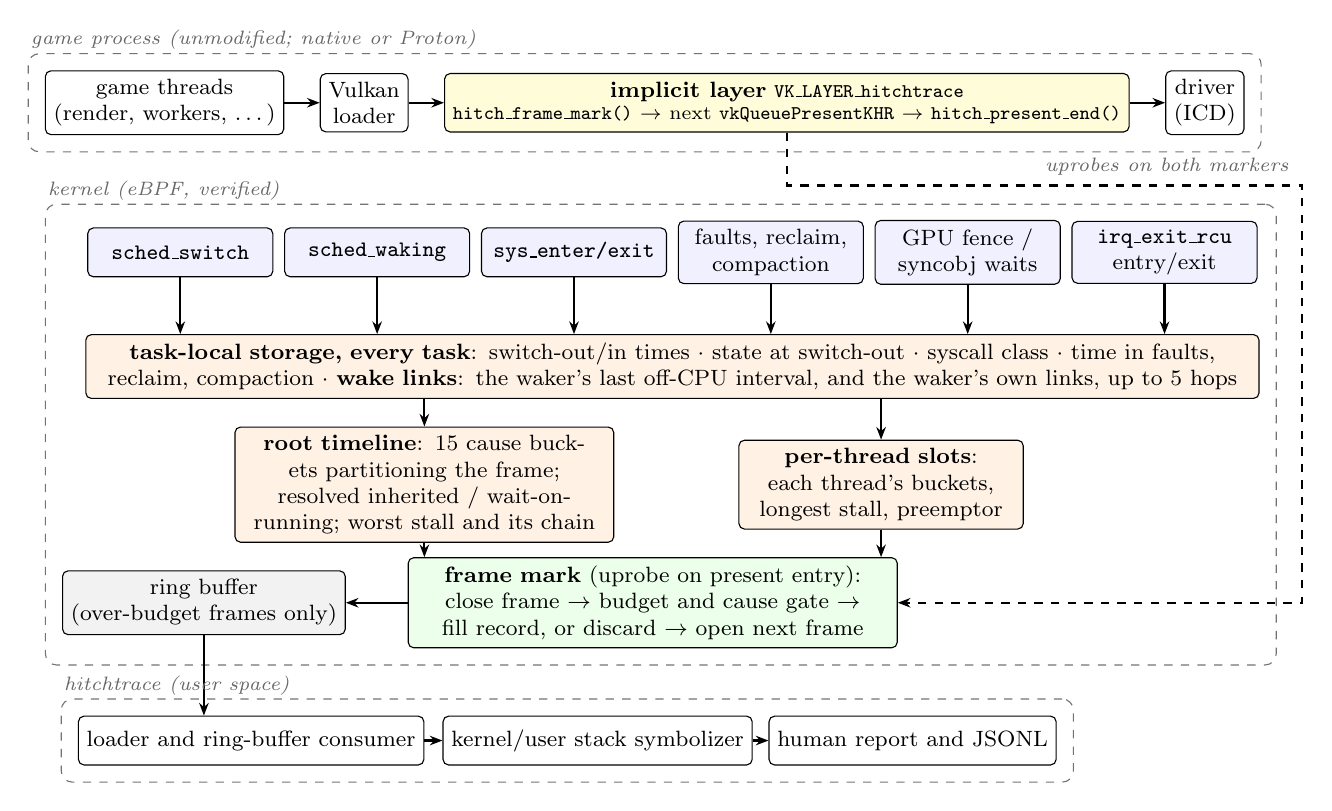
\begin{tikzpicture}[
  font=\footnotesize,
  box/.style={draw, rounded corners=2pt, align=center, inner sep=3pt, minimum height=0.62cm},
  hook/.style={box, fill=blue!6, minimum width=2.35cm},
  state/.style={box, fill=orange!10},
  prog/.style={box, fill=green!8},
  zone/.style={draw, dashed, rounded corners=4pt, inner sep=6pt, black!55},
  arr/.style={-{Stealth[length=1.6mm]}, thick},
  zlabel/.style={font=\scriptsize\itshape, text=black!60, anchor=south west, inner sep=1pt}
]
% ---- game process
\node[box] (threads) at (1.1,0) {game threads\\(render, workers, \ldots)};
\node[box, right=0.45cm of threads] (loader) {Vulkan\\loader};
\node[box, fill=yellow!15, right=0.45cm of loader, font=\scriptsize] (layer) {\textbf{\footnotesize implicit layer} \texttt{VK\_LAYER\_hitchtrace}\\\texttt{hitch\_frame\_mark()} $\to$ next \texttt{vkQueuePresentKHR} $\to$ \texttt{hitch\_present\_end()}};
\node[box, right=0.45cm of layer] (icd) {driver\\(ICD)};
\draw[arr] (threads) -- (loader);
\draw[arr] (loader) -- (layer);
\draw[arr] (layer) -- (icd);
\node[zone, fit=(threads)(icd)(layer)] (game) {};
\node[zlabel] at (game.north west) {game process (unmodified; native or Proton)};

% ---- hooks
\node[hook] (h1) at (1.3,-1.9) {\texttt{sched\_switch}};
\node[hook] (h2) at (3.8,-1.9) {\texttt{sched\_waking}};
\node[hook] (h3) at (6.3,-1.9) {\texttt{sys\_enter/exit}};
\node[hook] (h4) at (8.8,-1.9) {faults, reclaim,\\compaction};
\node[hook] (h5) at (11.3,-1.9) {GPU fence /\\syncobj waits};
\node[hook] (h6) at (13.8,-1.9) {\texttt{irq\_exit\_rcu}\\entry/exit};

% ---- task storage spans all hooks
\node[state, minimum width=14.9cm, text width=14.5cm] (ts) at (7.55,-3.35)
  {\textbf{task-local storage, every task}: switch-out/in times $\cdot$ state at switch-out $\cdot$ syscall class $\cdot$ time in faults, reclaim, compaction $\cdot$ \textbf{wake links}: the waker's last off-CPU interval, and the waker's own links, up to 5 hops};
\foreach \h in {h1,h2,h3,h4,h5,h6} \draw[arr] (\h.south) -- (\h.south |- ts.north);

% ---- per-frame state
\node[state, text width=4.6cm] (root) at (4.4,-4.85) {\textbf{root timeline}: 15 cause buckets partitioning the frame; resolved inherited / wait-on-running; worst stall and its chain};
\node[state, text width=3.4cm] (slots) at (10.2,-4.85) {\textbf{per-thread slots}: each thread's buckets, longest stall, preemptor};
\draw[arr] (root.north |- ts.south) -- (root.north);
\draw[arr] (slots.north |- ts.south) -- (slots.north);

% ---- frame mark program
\node[prog, text width=6.0cm] (mark) at (7.3,-6.35) {\textbf{frame mark} (uprobe on present entry): close frame $\to$ budget and cause gate $\to$ fill record, or discard $\to$ open next frame};
\draw[arr] (root.south) -- (root.south |- mark.north);
\draw[arr] (slots.south) -- (slots.south |- mark.north);
\draw[arr, dashed] (layer.south) -- (layer.south |- 0,-1.05) -- (15.55,-1.05) -- (15.55,-6.35) -- (mark.east);
\node[font=\scriptsize\itshape, text=black!60, anchor=south east] at (15.5,-1.05) {uprobes on both markers};

\node[box, fill=gray!10] (rb) at (1.6,-6.35) {ring buffer\\(over-budget frames only)};
\draw[arr] (mark.west) -- (rb.east);
\node[zone, fit=(h1)(h6)(ts)(root)(slots)(mark)(rb)] (kern) {};
\node[zlabel] at (kern.north west) {kernel (eBPF, verified)};

% ---- user space
\node[box] (fe) at (2.2,-8.1) {loader and ring-buffer consumer};
\node[box] (sym) at (6.6,-8.1) {kernel/user stack symbolizer};
\node[box] (out) at (10.6,-8.1) {human report and JSONL};
\draw[arr] (rb.south) -- (rb.south |- fe.north);
\draw[arr] (fe) -- (sym);
\draw[arr] (sym) -- (out);
\node[zone, fit=(fe)(out)] (usr) {};
\node[zlabel] at (usr.north west) {\sys (user space)};
\end{tikzpicture}}
\caption{Overview of \sys. Hooks keep per-task state current as the
scheduler runs; the frame mark closes the root thread's frame, evaluates the
gate, and emits a record only for an over-budget frame.}
\label{fig:arch}
\end{figure*}

Three principles guide the design.

\para{Account on the critical thread, not the process.}
Summing off-CPU time over all of a game's threads is unbounded: a process
with ten parked workers accumulates ten frames' worth of off-CPU time per
frame. \sys accounts on the \emph{root} thread, the thread that presents,
whose timeline within the frame is a partition of the frame time. Other
threads enter the record as context and through the chain.

\para{Build chains forward, not backward.}
Instead of recording wakeup edges and searching them when a frame goes bad,
every task carries the chain that led to its latest wakeup, copied forward
from its waker at wakeup time. The chain is always current, so resolving a
wait is a lookup, not a search.

\para{Decide at frame end, in the kernel.}
All per-frame state lives in maps until the frame mark. Only then does \sys
know whether the frame was over budget and how much of the overrun was
kernel-observable, and only then does it reserve ring-buffer space.

\subsection{Frame Source}
\label{sec:layer}

\sys needs two points per frame: present entry, which ends one frame and
begins the next, and present return, which ends the present call. The
implicit layer \texttt{VK\_LAYER\_hitchtrace} wraps
\texttt{vkQueuePresentKHR} in the device dispatch chain and calls two
exported, non-inlined marker functions around the next layer's present,
passing a process-global present counter as the frame id. \sys attaches a
uprobe to each marker in the layer's shared object. The layer is inert
unless \texttt{HITCHTRACE=1} is set; with no probe attached the markers are
two empty calls. Because the layer lives in the dispatch chain, it sees
presents from applications that bypass the loader (\S\ref{sec:background}),
and because Steam's container runtime resolves a host layer to the same
inode, a uprobe attached through the host path fires inside it.
\todo{Confirm inside pressure-vessel on the evaluation machine; the layer
is 64-bit only.}

For programs without a layer, \sys accepts any symbol in any binary as the
frame marker, and \texttt{-M ret:} brackets a single function with a
uprobe and a uretprobe.

\para{Frame model.} Frame $N$ runs from present entry $N-1$ to present entry
$N$. Blocked time of the root between present entry and present return is
charged to \bucket{block\_present}, the display pacing the application, so a
vsynced game does not register its vsync waits as stalls. The bracket is
only opened when the return probe is attached; otherwise a missed close
would silently relabel every wait.

\subsection{Root Timeline and Cause Taxonomy}
\label{sec:taxonomy}

Within a frame $[s, e)$, the root is always in one of four states, and every
interval of each state is clipped to the window:
\begin{equation*}
\textit{oncpu} + \textit{runnable} + \textit{runqueue} + \textstyle\sum \textit{blocked}_c = e - s .
\end{equation*}
On-CPU time is measured from switch-in to switch-out, never computed as a
remainder. At switch-out, \sys records the time, whether the switch was a
preemption, the task's \texttt{in\_iowait} bit, and a kernel stack for
voluntary sleeps. At switch-in, the interval since switch-out is split at
the wakeup timestamp: before the wakeup is blocked time, after it is
run-queue delay. Table~\ref{tab:taxonomy} lists the buckets and how each is
decided.

\begin{table}[t]
\centering
\footnotesize
\newcolumntype{L}[1]{>{\raggedright\arraybackslash}p{#1}}
\setlength{\tabcolsep}{3pt}
\begin{tabular}{@{}L{1.85cm}L{2.75cm}L{2.95cm}@{}}
\toprule
\textbf{Bucket} & \textbf{Hook} & \textbf{Rule} \\
\midrule
\bucket{oncpu} & \texttt{sched\_switch} & running, minus the carve-outs below \\
\bucket{oncpu\_fault}, \bucket{\ldots\_major} & fentry/fexit \texttt{handle\_\allowbreak mm\_\allowbreak fault} & on-CPU inside a fault; major from \texttt{VM\_FAULT\_\allowbreak MAJOR} \\
\bucket{oncpu\_\allowbreak reclaim} & direct and memcg reclaim tracepoints & on-CPU inside reclaim \\
\bucket{oncpu\_\allowbreak compact} & compaction tracepoints & on-CPU inside compaction \\
\midrule
\bucket{runnable} & \texttt{sched\_switch} & switched out while runnable; preemptor recorded \\
\bucket{runqueue} & \texttt{sched\_waking} & woken, waiting for a CPU \\
\midrule
\bucket{block\_\allowbreak present} & layer markers & blocked inside present \\
\bucket{block\_gpu} & \texttt{dma\_fence\_\allowbreak wait\_\allowbreak timeout}, \texttt{drm\_syncobj\_\allowbreak *wait\_\allowbreak ioctl} & blocked in a GPU fence wait \\
\bucket{block\_io} & \texttt{in\_iowait} at switch-out & blocked in I/O wait \\
\bucket{block\_futex} & \texttt{sys\_enter/\allowbreak exit} & in \texttt{futex}, \texttt{futex\_\allowbreak waitv}, \texttt{futex\_\allowbreak wait} \\
\bucket{block\_poll} & \texttt{sys\_enter/\allowbreak exit} & in poll, select, epoll \\
\bucket{block\_timer} & \texttt{sys\_enter/\allowbreak exit}, waker & in a sleep, or woken by an interrupt \\
\bucket{block\_task} & \texttt{sched\_waking} & woken by another task, none of the above \\
\bucket{block\_other} & --- & none of the above \\
\bottomrule
\end{tabular}
\caption{Root-timeline buckets, in the precedence order used for blocked
time. Together they partition the frame.}
\label{tab:taxonomy}
\end{table}

\para{What was asked beats who answered.} A blocked interval is named first
by what the thread asked the kernel for, and only then by who woke it: a
futex wait ended by its timeout interrupt is still a futex wait. The
present bracket outranks everything, including GPU fences, because a FIFO
present may legitimately block on a fence and blaming the GPU would point at
the application's own rendering.

\para{On-CPU kernel stalls.} Page faults, reclaim and compaction are mostly
on-CPU. \sys times them per task with entry/exit hooks and, at each
switch-out and at frame end, carves the time accrued since the last update
out of \bucket{oncpu}. Reclaim is hooked at both the direct and the memcg
tracepoints, since a cgroup memory limit triggers only the latter.

\para{Per-thread context.} Every thread of the target process also keeps a
per-frame line in one of 32 slots: its own buckets, its longest off-CPU
interval, the task that preempted it longest, and, if it is still off-CPU
when the frame closes, how long it has been waiting. These lines are context:
threads run in parallel, so their off-CPU time does not add to the frame.

\subsection{Online Wake-Chain Resolution}
\label{sec:chain}

\begin{figure}[t]
\centering
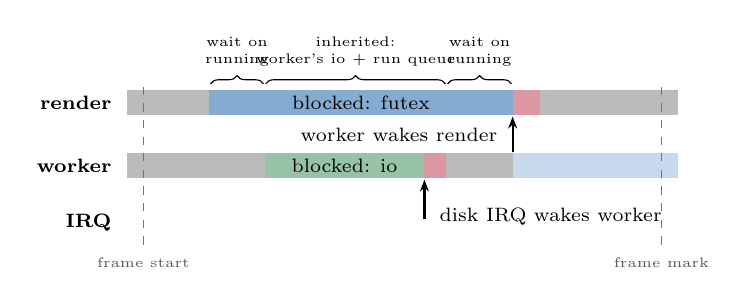
\begin{tikzpicture}[
  font=\scriptsize, x=0.7cm, y=0.8cm,
  arr/.style={-{Stealth[length=1.5mm]}, thick}
]
\def\lane#1#2{\node[anchor=east, font=\scriptsize\bfseries] at (-0.1,#1) {#2};}
\lane{2}{render}
\lane{1}{worker}
\lane{0.1}{IRQ}
% render (root)
\fill[cOncpu!70] (0,1.8) rectangle (1.5,2.2);
\fill[cFutex!55] (1.5,1.8) rectangle (7,2.2);
\fill[cSched!45] (7,1.8) rectangle (7.5,2.2);
\fill[cOncpu!70] (7.5,1.8) rectangle (10,2.2);
\node at (4.25,2) {blocked: futex};
% worker
\fill[cOncpu!70] (0,0.8) rectangle (2.5,1.2);
\fill[cIO!45] (2.5,0.8) rectangle (5.4,1.2);
\fill[cSched!45] (5.4,0.8) rectangle (5.8,1.2);
\fill[cOncpu!70] (5.8,0.8) rectangle (7,1.2);
\fill[cFutex!25] (7,0.8) rectangle (10,1.2);
\node at (3.95,1) {blocked: io};
% wakeups
\draw[arr] (5.4,0.15) -- (5.4,0.78);
\node[anchor=west] at (5.5,0.2) {disk IRQ wakes worker};
\draw[arr] (7,1.22) -- (7,1.78);
\node[anchor=east] at (6.9,1.5) {worker wakes render};
% frame window
\draw[black!55, dashed] (0.3,-0.25) -- (0.3,2.3);
\draw[black!55, dashed] (9.7,-0.25) -- (9.7,2.3);
\node[font=\tiny, text=black!65, anchor=north] at (0.3,-0.3) {frame start};
\node[font=\tiny, text=black!65, anchor=north] at (9.7,-0.3) {frame mark};
% resolution of render's blocked interval [1.5, 7)
\draw[decorate, decoration={brace, amplitude=3pt}] (1.52,2.3) -- (2.48,2.3)
  node[midway, above=3pt, align=center, font=\tiny] {wait on\\running};
\draw[decorate, decoration={brace, amplitude=3pt}] (2.52,2.3) -- (5.78,2.3)
  node[midway, above=3pt, align=center, font=\tiny] {inherited:\\worker's io + run queue};
\draw[decorate, decoration={brace, amplitude=3pt}] (5.82,2.3) -- (6.98,2.3)
  node[midway, above=3pt, align=center, font=\tiny] {wait on\\running};
\end{tikzpicture}
\caption{Resolving a blocked interval of the root. The part of render's
futex wait that overlaps the worker's own off-CPU interval (I/O plus
run queue, ended by the disk interrupt) is inherited; the rest is time the
worker spent running, i.e.\ render waiting for work. The reported chain is
render $\leftarrow$ worker (io) $\leftarrow$ [irq].}
\label{fig:chain}
\end{figure}

\para{Copy-forward chains.} On every \texttt{sched\_waking}, \sys writes into
the wakee's task storage a \emph{link} describing the waker as it is at that
moment: its identity and the bounds and cause of its most recent completed
off-CPU interval. It then copies the waker's own links into the wakee's
slots $1..4$, so the wakee holds its waker, its waker's waker, and so on, up
to five hops. The copy has constant size, as the verifier requires, and a
sequence counter on the waker detects a copy torn by a concurrent wakeup of
the waker on another CPU; a torn copy is discarded rather than trusted.

\para{Resolution.} When the root switches back in after a blocked interval
$[\textit{lo}, \textit{hi})$ ended by another task,
\begin{align*}
\textit{inherited} &= \bigl|[\textit{lo}, \textit{hi}) \cap [w_\textit{out}, w_\textit{in})\bigr|,\\
\textit{wait\_oncpu} &= (\textit{hi} - \textit{lo}) - \textit{inherited},
\end{align*}
where $[w_\textit{out}, w_\textit{in})$ is the waker's last off-CPU interval
as recorded in the link (Figure~\ref{fig:chain}). Inherited time is a stall
one hop away; \textit{wait\_oncpu} is the root waiting for a thread that was
running, the game's own work rather than a kernel stall. Both are reported
alongside the partition. For the frame's longest blocked interval, \sys
repeats the overlap hop by hop down the chain, recording for each hop the
task, the time it explains, what it was blocked in, and whether its interval
had already ended before the previous hop's began (a stale link).

\para{Where chains stop.} A chain ends at an interrupt, at the idle task, or
at a waker that was running. \sys detects hardirq and NMI context from the
per-CPU preemption count, read through two weak kernel symbols because x86
moved the variable into and back out of a per-CPU structure between kernel
versions; the verifier prunes the branch for the symbol that does not exist.
Softirqs that run on interrupt exit, after the hardirq bits are cleared, are
detected by a per-CPU nesting counter maintained by \texttt{fentry} and
\texttt{fexit} on \texttt{irq\_exit\_rcu} and reset at every context switch,
where it must be zero. An interrupt link carries no task identity: the task
it names is a bystander.

\subsection{Cause Gate and Emission}
\label{sec:gate}

At the frame mark, \sys closes the root's on-CPU tail, applies the
carve-outs, and computes the frame time $f$ and the budget $b$. The budget is
fixed, or, for an uncapped game, 1.5 times the rolling median of the last 19
frames, with a floor. The frame is a hitch if $f > b$. With a share $\sigma
> 0$, the frame is emitted only if
\[
\textit{stall} \geq \sigma \cdot (f - b),
\]
where \textit{stall} is the root's time in every bucket except
\bucket{oncpu} and \bucket{block\_present}. A share of zero gates on the
symptom alone, which is what an unbiased prevalence study needs; a share of
0.5 says ``at least half of the overrun must be kernel-observable.''

For an emitted frame, \sys reserves a 6,896-byte record in the ring buffer
and fills it with the partition, the resolution totals, the worst stall and
its chain, and the 32 per-thread lines. For every other frame it resets the
root's state and moves on: no bytes cross into user space. The user-space
front end symbolizes kernel stacks, optionally user stacks, and writes a
human-readable report and JSONL. Figure~\ref{fig:record} shows a record.

\begin{figure*}[t]
\centering
\begin{lrbox}{\recordbox}
\footnotesize
\begin{minipage}{1.38\textwidth}
\begin{verbatim}
hitch frame 180  32.8 ms  (budget 16.7 ms, over by 16.1 ms)  root hb_root/67200  [open stall]
  oncpu      3.7 ms   runqueue 0.0 ms
  blocked   29.0 ms  futex 20.3 | present 8.7
  resolved   waiting on a running task 0.1 ms, inherited stalls 20.3 ms
  worst stall 20.3 ms  blocked in __futex_wait
    <- hb_worker/67195   blocked 20.3 ms in anon_pipe_read
      <- hb_feeder/67196 blocked 20.1 ms in do_nanosleep
        <- [hardirq]     woken by an interrupt
  threads
    hb_root/67200    (root)  oncpu 3.7  runqueue 0.0  blocked 29.0 futex 20.3 | present 8.7
    hb_worker/67195          oncpu 0.0  runqueue 0.1  blocked 32.6 futex 12.4 | task 20.2 (still blocked at frame end 0.0 ms)   largest 20.3 ms in anon_pipe_read
    hb_feeder/67196          oncpu 0.0  runqueue 0.1  blocked 32.5 futex 12.4 | timer 20.1 (still blocked at frame end 0.1 ms)   largest 20.1 ms in do_nanosleep
  2 stalls this frame
\end{verbatim}
\end{minipage}
\end{lrbox}
\resizebox{\textwidth}{!}{\usebox{\recordbox}}
\caption{A \sys record, verbatim, for an injected \texttt{worker\_block}
frame of \bench. The root's 20.3\,ms futex wait is inherited in full from the
worker, which was blocked reading a pipe, which in turn waited on the
feeder's sleep, ended by a timer interrupt. The same record is written as
JSONL.}
\label{fig:record}
\end{figure*}

\subsection{Implementing Under the Verifier}
\label{sec:verifier}

Expressing this design as verified BPF required several restructurings,
which we report because they are the practical cost of in-kernel
attribution.

\para{Per-thread slots by index, not by counter.} The emit path copies up to
32 per-thread lines into the record in a bounded loop that the verifier
unrolls. Writing each thread at a running output index made every path
through the unrolled loop distinct, the verifier could not prune states, and
the program exceeded the one-million-instruction limit. Each thread instead
lands at its own fixed slot index; unused slots are zeroed and skipped in
user space. The root's own slot is finalized before the loop for the same
reason.

\para{State in task storage.} All per-task state lives in task-local
storage, created lazily and freed with the task. A fixed-size hash keyed by
thread id, as in earlier chain tools, both overflows and leaks entries of
exited tasks.

\para{Constant-size copies and bounded selection.} The chain copy always
moves four links and trims logically; the rolling median is a counting
selection over two bounded loops rather than a sort.

\para{Attach order.} Paired entry and exit hooks attach exit first, so an
invocation in flight during attachment can produce only an unmatched
decrement, which is ignored, never a counter stuck high. The present-return
probe attaches before the frame marker, so no frame can open a present
bracket that nothing can close.

\subsection{Discussion and Limitations}
\label{sec:limitations}

\para{One root per frame.} Under DXVK and vkd3d-proton the presenting thread
is a translation thread, and a stall on the game thread can close in the
frame before the late one when frames are pipelined. The chain reaches the
game thread when the present thread's waits are ended by it, but the
prototype does not yet look back across a frame boundary.
\todo{Measure on Proton titles; consider identifying the frame thread from
the chain at present.}

\para{The worst stall is one interval.} The chain is resolved for the
frame's longest single blocked interval. A fragmented stall (an I/O split
into many short waits) or a stall that is not a blocked interval at all
(preemption, on-CPU faults) cannot win, and a benign contiguous sleep can
(\S\ref{sec:eval-app}). Aggregate accounting is unaffected; only the choice
of which interval to explain is.

\para{The gate does not yet use the resolution.} The share gate weighs
blocked time including \textit{wait\_oncpu}. Section~\ref{sec:eval-gate}
shows the consequence and that subtracting it fixes it.

\para{Not yet recorded.} The requested duration of a sleep, so that an
oversleeping frame limiter is distinguishable from an intentional sleep;
the task occupying the CPU during a run-queue wait; and a refinement of
\bucket{block\_other} by kernel stack (e.g.\ the ntsync driver~\cite{ntsync},
split-lock mitigation~\cite{lwn-splitlock}). \todo{Implement or scope out.}

%-------------------------------------------------------------------------------
\section{Evaluation}
\label{sec:eval}
%-------------------------------------------------------------------------------

We evaluate \sys by asking:
\begin{enumerate}[label=\textbf{Q\arabic*}]
\item Does \sys record exactly the over-budget frames? (\S\ref{sec:eval-accuracy})
\item Does the partition attribute an injected stall to the right cause? (\S\ref{sec:eval-accuracy})
\item Does chain resolution separate kernel stalls from waiting on work? (\S\ref{sec:eval-chain})
\item Does frame-scoped accounting capture hitches made of many small stalls? (\S\ref{sec:eval-cuts})
\item Does the cause gate reject hitches that are not kernel-observable? (\S\ref{sec:eval-gate})
\item Does \sys work on a real Vulkan application? (\S\ref{sec:eval-app})
\item What does always-on tracing cost, and how does output scale? (\S\ref{sec:eval-overhead})
\item How common are kernel-observable hitches in Linux games? (\S\ref{sec:eval-prevalence})
\end{enumerate}

\para{Setup.} The results in this draft come from a development virtual
machine: Hyper-V on an Intel Core i7-12700H host, 10 vCPUs, 7\,GB of memory,
Ubuntu 24.04.5 with Linux 7.0.0-31-generic (\texttt{PREEMPT\_LAZY}), and
Mesa 25.2.8 with lavapipe~\cite{lavapipe}, the only Vulkan device the VM
exposes. The VM has no PMU. Its timing is not representative of a gaming
machine, so we use it only for questions whose answer does not depend on
absolute timing (Q1--Q6). Q7 and Q8 require bare metal with a GPU and are
planned on \tbd{[evaluation machine: AMD Ryzen 7 PRO 8700GE with Radeon 780M,
Deck-class limits imposed with cgroups]}.

\subsection{Frame Capture and Attribution Accuracy}
\label{sec:eval-accuracy}

\para{Benchmark.} \bench is a synthetic game loop. Its root thread burns a
calibrated slice of CPU each frame, hands a job to a worker and waits for it
on a futex, then presents: the frame marker is called at present entry, the
thread sleeps to the frame deadline, and the present-return marker is called
after. The loop paces to 14.6\,ms so that healthy frames stay under a
16.7\,ms budget. Every twentieth frame it runs one injector that stalls the
frame through a single kernel mechanism, and it logs every frame's id,
duration, injection and expected bucket as JSON. We run each of
\hbnClasses\ injector classes and one uninjected baseline for eight seconds
with \sys attached for five, and join records to ground truth on frame id.
Frames that straddle the start or end of tracing are excluded.

\begin{table*}[t]
\centering
\footnotesize
\setlength{\tabcolsep}{3.5pt}
\begin{tabular}{@{}llcccccccc@{}}
\toprule
 & & \textbf{Expected} & \textbf{Recorded /} & \textbf{Largest bucket} & \textbf{Worst stall /} & \multicolumn{2}{c}{\textbf{Share gate (prototype)}} & \multicolumn{2}{c}{\textbf{Resolved gate}} \\
\cmidrule(lr){7-8}\cmidrule(l){9-10}
\textbf{Class} & \textbf{Injection} & \textbf{bucket} & \textbf{injected} & \textbf{= expected} & \textbf{excess} & \textbf{share} & \textbf{pass $\geq$0.5} & \textbf{share} & \textbf{pass $\geq$0.5} \\
\midrule
\hbTableRows
\bottomrule
\end{tabular}
\caption{Attribution on \bench (medians over injected frames). \emph{Worst
stall / excess}: the single longest blocked interval as a fraction of the
frame's overrun. \emph{Share}: the root's kernel-observable time (all buckets
but \bucket{oncpu} and \bucket{block\_present}) over the overrun, as the
in-kernel gate computes it. \emph{Resolved gate}: the same with time spent
waiting on a running task subtracted, computed offline from the records.
Generated by \texttt{scripts/hitchbench\_results.py}.}
\label{tab:bench}
\end{table*}

\para{Q1: exactly the over-budget frames.} Across the twelve runs, \bench
logged \hbtotFrames\ fully traced frames, of which \hbtotOver\ exceeded the
budget. \sys emitted exactly one record for each of them and none for any
frame within budget (\hbtotMiss\ missed, \hbtotExtra\ extra). Its frame
times agree with \bench's own to within \hbmaxDtUs\,$\mu$s. In the
uninjected baseline, \hbbaselineRecords\ of \hbbaselineFrames\ frames
exceeded the budget and was recorded.

\para{Q2: the right cause.} Table~\ref{tab:bench} and
Figure~\ref{fig:breakdown} show the result per class. Every injected frame
was recorded, and the largest bucket of the root's partition named the
injected mechanism in \hbtotMatch\ of \hbtotInj. The two classes that fall
short are informative rather than wrong. In \texttt{fault}, the injector
touches a burst of fresh pages; \sys carves a median \hbfaultoncpufault\,ms
out of on-CPU time as \bucket{oncpu\_fault}, but the loop that touches the
pages runs \hbfaultoncpu\,ms of user code of its own, so plain
\bucket{oncpu} stays larger. In \texttt{io}, the cold read spends a median
\hbioblockio\,ms in I/O wait but also \hbiooncpu\,ms on-CPU copying from the
page cache, and in 6 of 16 frames the present wait that follows exceeds the
I/O. In both cases the mechanism is present in the record at its real size;
``largest bucket'' is too blunt a criterion. \todo{Adopt the per-level
diagnosis criterion (injected bucket $\geq X$\% of excess above the
normal-frame baseline) and use \texttt{O\_DIRECT} for the I/O injector.}

\begin{figure}[t]
\centering
\pgfplotstableread{data/hitchbench_breakdown.dat}\breakdown
\begin{tikzpicture}
\begin{axis}[
  xbar stacked,
  width=0.93\columnwidth, height=6.4cm,
  bar width=6.5pt,
  y dir=reverse,
  ytick=data,
  yticklabels from table={\breakdown}{class},
  yticklabel style={font=\ttfamily\scriptsize},
  xticklabel style={font=\scriptsize},
  xlabel={Mean time per injected frame (ms)},
  xlabel style={font=\scriptsize},
  xmin=0, xmax=45,
  enlarge y limits=0.06,
  set layers,
  legend cell align=left,
  legend style={font=\scriptsize, at={(0.5,1.02)}, anchor=south,
    legend columns=5, draw=none, /tikz/every even column/.append style={column sep=4pt}},
  legend image code/.code={\draw[#1, draw=none] (0cm,-0.08cm) rectangle (0.25cm,0.1cm);},
  axis x line*=bottom, axis y line*=left,
  xmajorgrids, grid style={black!12},
]
\addplot[fill=cOncpu, draw=none] table[x=oncpu, y expr=\coordindex]{\breakdown};
\addplot[fill=cOncpuK, draw=none] table[x=oncpukern, y expr=\coordindex]{\breakdown};
\addplot[fill=cSched, draw=none] table[x=sched, y expr=\coordindex]{\breakdown};
\addplot[fill=cFutex, draw=none] table[x=futex, y expr=\coordindex]{\breakdown};
\addplot[fill=cPoll, draw=none] table[x=poll, y expr=\coordindex]{\breakdown};
\addplot[fill=cIO, draw=none] table[x=io, y expr=\coordindex]{\breakdown};
\addplot[fill=cTimer, draw=none] table[x=timer, y expr=\coordindex]{\breakdown};
\addplot[fill=cPresent, draw=black!30] table[x=present, y expr=\coordindex]{\breakdown};
\addplot[fill=cOther, draw=none] table[x=other, y expr=\coordindex]{\breakdown};
\legend{oncpu, oncpu kernel, runnable+rq, futex, poll, io, timer, present, other}
\draw[on layer=axis foreground, black, dashed, thick] (axis cs:16.667,-0.6) -- (axis cs:16.667,10.6);
\end{axis}
\end{tikzpicture}
\caption{Composition of the root's frame for each injector class (mean over
injected frames). Each bar sums to the frame time; the dashed line is the
16.7\,ms budget.}
\label{fig:breakdown}
\end{figure}

\subsection{Chain Resolution}
\label{sec:eval-chain}

\para{Q3.} Two classes produce the same symptom on the root, a futex wait of
about 20\,ms on the worker, for opposite reasons. In
\texttt{worker\_block} the worker is itself blocked, reading a pipe that a
feeder thread writes after a 20\,ms sleep. In \texttt{worker\_cpu} the worker
simply computes for 20\,ms. By bucket the two are indistinguishable
(Table~\ref{tab:bench}). By resolution they are opposites: for
\texttt{worker\_block}, a median \hbworkerblockInherited\,ms of the wait is
inherited and \hbworkerblockWaitOncpu\,ms is waiting on a running task; for
\texttt{worker\_cpu}, \hbworkercpuInherited\,ms and \hbworkercpuWaitOncpu\,ms.
The chain for \texttt{worker\_block} is
\hbworkerblockChain\ in \hbworkerblockChainN\ frames: the worker, the feeder
the worker was waiting on, and the timer interrupt that ended the feeder's
sleep. For \texttt{poll}, where the root waits in \texttt{epoll\_wait} for
the feeder directly, \hbpollInherited\,ms is inherited through
\hbpollChain.

This is the distinction a per-cause total cannot make and the reason \sys
resolves waits online: a futex wait on a stalled thread is a kernel stall
one hop away, while a futex wait on a busy thread is the game's own CPU
work, out of scope, and should not count as a kernel stall.

\subsection{Hitches Made of Many Small Stalls}
\label{sec:eval-cuts}

\para{Q4.} The \texttt{thousand\_cuts} injector makes the root sleep
about forty times for 0.5\,ms each. Every injected frame was recorded with
the timer bucket largest, a median of \hbthousandcutsNstalls\ stalls in the
frame, and a longest single stall covering only \hbthousandcutsWorstFrac\
of the overrun, against 1.09--1.26 for the single-stall classes. A per-event
filter at any threshold above 0.5\,ms emits nothing for these frames by
construction, and one below it emits a comparable stream for every normal
frame. \todo{Run \texttt{perf record --off-cpu --off-cpu-thresh} and the
ftrace per-stall synthetic event on the same schedule and report capture
rate vs.\ threshold (M2), and sweep stall size and count.}

\subsection{Cause Gating}
\label{sec:eval-gate}

\para{Q5.} Two classes are negative controls, over budget for reasons that
are not kernel stalls: \texttt{cpu\_spike} burns 25\,ms of CPU on the root,
and \texttt{present\_long} lengthens the present wait. The prototype's gate
at $\sigma=0.5$ rejects both in every frame (median share
\hbcpuspikeShare\ and \hbpresentlongShare) and passes every positive class.
It also passes \texttt{worker\_cpu} (share \hbworkercpuShare), because the
gate counts the root's futex wait whether or not the thread it waited for
was stalled. Subtracting the resolved \textit{wait\_oncpu} time, which \sys
already computes, drops \texttt{worker\_cpu} to \hbworkercpuRShare\ and
rejects it in every frame (\hbworkercpuRGated\ pass) while every positive
class still passes (Table~\ref{tab:bench}, last column).
\todo{Move the resolved gate into the BPF program and re-run.}

\para{vkcube.} We also ran \sys on \texttt{vkcube-wayland} under lavapipe,
which rasterizes inside the present call. With the present bracket and no
cause gate, 98 of 210 frames (46.7\%) exceeded 16.7\,ms; in their records
96.8\% of the time was \bucket{block\_present}, with \texttt{gnome-shell}
named as the waker in 97 of 98, and a median of only 12\% of the overrun was
kernel-observable. With $\sigma=0.5$, 25 of 479 frames (5.2\%) were emitted.
Without the bracket, the same waits appear as \bucket{block\_poll} (86\% of
recorded time) in every one of 223 records: the bracket is what keeps
display pacing from being reported as a stall. The frames that survive the
gate have a median overrun of only 147\,$\mu$s, sub-millisecond jitter that
passes a ratio test easily because the denominator is tiny.
\todo{Add a minimum-overrun floor to the gate.}

\subsection{A Real Vulkan Application}
\label{sec:eval-app}

\para{Q6.} \todo{Rebuild the test game and re-run; the artifacts of the
first run were lost. Numbers below are from that run (session notes) and
must be regenerated before submission.} We wrote a small asteroids-style
Vulkan game in C with six named threads: render and simulation threads that
hand off every frame over a futex, an asset streamer doing real file I/O
with \texttt{O\_DIRECT}, a timer tick, and CPU hogs. It paces itself with a
sleep and gets its frame marks from the layer, with no instrumentation of its
own. Seven injectors fire round-robin every 20--30 frames. With a
22\,ms budget, \sys emitted \tbd{44} records over \tbd{1,097} frames; all
\tbd{43} injections were caught, each with the predicted bucket largest, and
one uninjected frame was over budget. The asset injection's record resolves
the render thread's 47.5\,ms futex wait through the streamer's
\texttt{blk\_io\_schedule} to the block-device completion interrupt.

The same run exposed the limitation of \S\ref{sec:limitations}: in
\tbd{15} of \tbd{44} records the worst stall, and hence the chain, was the
game's own frame-limiter sleep rather than the injected cause. Preemption
and on-CPU faults are never candidates, and the I/O injector's 25\,ms of
I/O wait arrived in 132 intervals whose longest (8\,ms) lost to a
contiguous 4.3\,ms pacing sleep half the time. The partition was correct in
every case; only the choice of which interval to explain was not.
\todo{Rank worst-stall candidates by summed time per (bucket, waker) and admit
\bucket{runnable} and on-CPU carve-outs; re-run.}

\subsection{Overhead and Output Volume}
\label{sec:eval-overhead}

\para{Q7.} \todo{Not yet measured. Plan (M3): same workload (\bench steady
state and one title's benchmark loop), same cgroup limits, $\geq$5 runs each,
for no tool, \sys ($\sigma=0$ and $0.5$), an ftrace flight recorder with a
present-triggered snapshot, \texttt{perf --off-cpu}, delay accounting polled
at present, and systing~\cite{systing}. Report $\Delta$p99 frame time and
$\Delta$1\% low against no tool, tool CPU, and bytes per hour at controlled
hitch rates of 0.01, 0.1 and 1 per second, plus snapshot drain time and
dropped snapshots. Report the result whichever tool wins on perturbation.}
Preliminary observations: on the test game, presents per second were 57.6
untraced and 57.7--58.0 traced, and the clean-frame median was unchanged at
16.68\,ms \tbd{(VM, lavapipe; not representative)}. A record is 6,896 bytes,
so at one hitch per second \sys emits about 24.8\,MB per hour, and nothing
for frames within budget.

\subsection{Prevalence in Linux Games}
\label{sec:eval-prevalence}

\para{Q8.} \todo{Not yet measured. Plan (M0): \tbd{5} titles (Proton and
native) $\times$ 3 conditions (unconstrained; Deck-class cgroup limits;
Deck-class plus a background download and a cold shader cache), $\geq$45
minutes each, $\sigma=0$ so every over-budget frame is recorded. Report the
distribution of kernel-observable share of the overrun, resolved as in
\S\ref{sec:eval-gate}; the breakdown by bucket; and the split between
game-initiated waits and external causes. This number has not been
published for Linux games and is the paper's motivating measurement either
way it comes out.}

%-------------------------------------------------------------------------------
\section{Related Work}
\label{sec:related}
%-------------------------------------------------------------------------------

\para{Triggered and retroactive capture.} Deciding after the fact what to
keep is an old idea: DTrace aggregations and speculative
tracing~\cite{cantrill2004dtrace}, latency-tracker with LTTng
snapshots~\cite{desfossez2016latency,lttng}, ftrace histogram triggers and
snapshots~\cite{ftracehist}, rtla~\cite{rtla}, Perfetto's
triggers~\cite{perfetto-triggers}, and Hindsight's retroactive sampling for
distributed systems~\cite{zhang2023hindsight}. \sys adopts the pattern; what
it adds is a trigger that depends on cause as well as symptom and a record
computed in the kernel instead of a raw window.

\para{Off-CPU and critical-path analysis.} Off-CPU, off-wake and chain-graph
analysis~\cite{gregg-offcpu,gregg-chaingraph,gregg2019bpf} attribute blocked
time to stacks and wakers, in aggregate. Critical-path
analysis~\cite{giraldeau2016wait,zhou2018wperf,perfetto-critpath} and wait
analysis on Windows~\cite{ets-wait-analysis} follow waits across threads
precisely, offline. \sys executes a bounded, online version of the same
analysis, scoped to one frame and run only when the frame goes bad.

\para{Accounting per unit of work.} Linux delay accounting and PSI
accumulate stall time by cause per task and system-wide~\cite{delayacct,psi}.
VarMRI accumulates kernel and hardware events per server request and emits
one record per request, using a kernel patch~\cite{varmri}. \sys applies
per-unit accounting to frames, adds the waker and the chain, and runs as
verified BPF on a stock kernel.

\para{Frame-aware profilers.} Nsight Systems delimits Vulkan frames at the
present call and flags actions whose per-frame time far exceeds a rolling
median~\cite{nsight}; Perfetto's FrameTimeline classifies jank on
Android~\cite{perfetto-frametimeline} and AOSP relies on a blocked-reason
tracepoint that upstream kernels lack~\cite{aosp-blocked-reason}; hwui\_mon
and frame-analyzer detect Android frames with
uprobes~\cite{hwui-mon,frame-analyzer}; Tracy~\cite{tracy} and
Superluminal~\cite{superluminal} need instrumentation or full captures;
PresentMon and MangoHud measure frame times without
causes~\cite{presentmon,mangohud}. None of them attributes frames to kernel
causes online.

\para{Linux gaming tooling.} systing records all scheduling events of a
system or process into Perfetto or DuckDB and is used by sched\_ext
developers~\cite{systing}; VaporMark post-processes \texttt{perf sched}
traces to evaluate schedulers~\cite{vapormark,scx}. \sys is complementary:
its records are compact enough to leave running for a session and could be
exported into those tools' formats.

%-------------------------------------------------------------------------------
\section{Conclusion}
%-------------------------------------------------------------------------------

This paper presented \sys, which explains frame hitches in unmodified Linux
games by partitioning the presenting thread's frame by kernel cause,
resolving its waits online through wake chains carried in task-local
storage, and deciding in the kernel, at frame end, whether the frame is
worth a record. On a ground-truth benchmark it recorded exactly the
over-budget frames, named the injected mechanism, and distinguished a
thread waiting on a stalled worker from one waiting on a busy worker.
\tbd{[Conclusion on real titles, overhead and prevalence.]}

%-------------------------------------------------------------------------------
\section*{Acknowledgments}
%-------------------------------------------------------------------------------

\todo{Acknowledgments and funding.}

%-------------------------------------------------------------------------------
\section*{Availability}
%-------------------------------------------------------------------------------

\todo{Repository URL, license, and the scripts that regenerate every table
and figure from raw runs.}

%-------------------------------------------------------------------------------
\bibliographystyle{plain}
\bibliography{references}

\end{document}
